%&pdflatex
\documentclass{standalone}
\usepackage{tikz}
\usetikzlibrary{arrows}
\usetikzlibrary{shapes}
\usetikzlibrary{positioning}
\usetikzlibrary{snakes}

\begin{document}

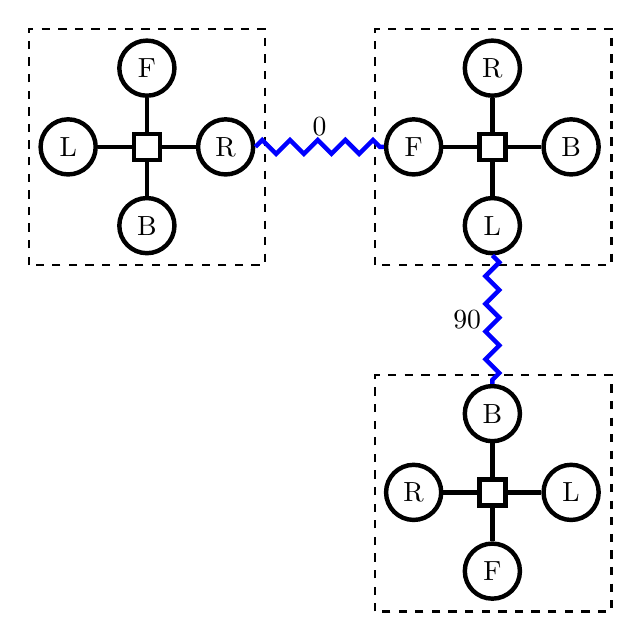
\begin{tikzpicture}
    \node [draw, ultra thick, regular polygon,regular polygon sides=4] (body) {};
    \node [draw, ultra thick, circle, right of=body, minimum size=0.7cm] (right) {R};
    \node [draw, ultra thick, circle, left of=body, minimum size=0.7cm] (left) {L};
    \node [draw, ultra thick, circle, below of=body, minimum size=0.7cm] (back) {B};
    \node [draw, ultra thick, circle, above of=body, minimum size=0.7cm] (front) {F};
    \draw [thick, dashed] (-1.5,-1.5) rectangle ++ (3,3);
    
    \node [draw, ultra thick, regular polygon,regular polygon sides=4, right = 4cm of body] (body1) {};
    \node [draw, ultra thick, circle, above of=body1, minimum size=0.7cm] (right1) {R};
    \node [draw, ultra thick, circle, below of=body1, minimum size=0.7cm] (left1) {L};
    \node [draw, ultra thick, circle, right of=body1, minimum size=0.7cm] (back1) {B};
    \node [draw, ultra thick, circle, left of=body1, minimum size=0.7cm] (front1) {F};
    \draw [thick, dashed] (2.9,-1.5) rectangle ++ (3,3);
    
    \node [draw, ultra thick, regular polygon,regular polygon sides=4, below = 4cm of body1] (body2) {};
    \node [draw, ultra thick, circle, left of=body2, minimum size=0.7cm] (right2) {R};
    \node [draw, ultra thick, circle, right of=body2, minimum size=0.7cm] (left2) {L};
    \node [draw, ultra thick, circle, above of=body2, minimum size=0.7cm] (back2) {B};
    \node [draw, ultra thick, circle, below of=body2, minimum size=0.7cm] (front2) {F};
    \draw [thick, dashed] (2.9,-5.9) rectangle ++ (3,3);
    
    \draw [ultra thick] (body) -- (right);
    \draw [ultra thick] (body) -- (left);
    \draw [ultra thick] (body) -- (back);
    \draw [ultra thick] (body) -- (front);
    
    \draw [ultra thick] (body1) -- (right1);
    \draw [ultra thick] (body1) -- (left1);
    \draw [ultra thick] (body1) -- (back1);
    \draw [ultra thick] (body1) -- (front1);
    
    \draw [ultra thick] (body2) -- (right2);
    \draw [ultra thick] (body2) -- (left2);
    \draw [ultra thick] (body2) -- (back2);
    \draw [ultra thick] (body2) -- (front2);
    
    \draw [ultra thick, draw=blue, snake=zigzag] (right) -- node[anchor=south]{0} (front1) ;
    \draw [ultra thick, draw=blue, snake=zigzag] (left1) -- node[anchor=east]{90} (back2) ;
    
\end{tikzpicture}

\end{document}



